\documentclass[a4paper,11pt,twocolumn]{article}
%\documentclass[twocolumn,aps,pre,groupedaddress]{revtex4-1}

\usepackage{amsmath}
\usepackage{graphicx}
\usepackage{amsmath}
\usepackage{graphicx}
\usepackage{subfig}
\usepackage{epstopdf}
\usepackage{amssymb}

\begin{document}
\title{Time Series Leanings}
\author{James M. McCracken}
%\email{jmccrac1@masonlive.gmu.edu}
%\affiliation{School of Physics, Astronomy, and Computational Sciences \\ George Mason University \\ 4400 University Drive MS 3F3, Fairfax,VA. 22030-4444}
\author{Robert S. Weigel}
%\email{rweigel@gmu.edu}
%\affiliation{School of Physics, Astronomy, and Computational Sciences \\ George Mason University \\ 4400 University Drive MS 3F3, Fairfax,VA. 22030-4444}
\date{\today}

%\begin{abstract}
%\end{abstract}

%\pacs{}
\maketitle

\section{Introduction}

\section{Causal Penchant}
Define the {\em causal penchant} as
\begin{equation}
\label{eq:pen}
\rho_{EC} := P\left(E|C\right) - P\left(E|\bar{C}\right)\;\;.
\end{equation}
The motivation for this expression is in te interpretation of $\rho_{EC}$ as a causal indicator; i.e.\ if $C$ causes (or {\em drives}) $E$, then $\rho_{EC} > 0$, and if $\rho_{EC} \le 0$, then the direction of causal influence in the system is undetermined.  If the effect $E$ is assumed to be recorded in one time series and the cause $C$ is assumed to be recorded in a different time series, then the direction of causal influence in the system can be determined by comparing various penchants calculated using both time series.  The details of these comparison is discuss in the following sections, but some potential philosophical issues with this definition will be addressed first.

$\ldots$ {\em {\bf Add discussion of Pearl argument that $P(E|\bar{C})$ is ''unobservable''.}}

Pearl's concerns can be addressed by rewriting Eqn.\ \ref{eq:pen} using the law of total probability, i.e
\begin{equation}
\label{eq:totp}
P(E) = P(E|C)P(C) + P(E|\bar{C})P(\bar{C})\;\;,
\end{equation}
or Bayes theorem, i.e.\ 
\begin{equation}
\label{eq:bayes}
P(E|\bar{C}) = P(\bar{C}|E)\frac{P(E)}{P(\bar{C})}\;\;.
\end{equation}
The definition of probability complements implies $P(\bar{C}) = 1-P(C)$ and $P(\bar{C}|E) = 1-P(C|E)$.  Applying Eqn.\ \ref{eq:bayes} leads to
\begin{equation}
P(\bar{C}|E) = 1-P(E|C)\frac{P(C)}{P(E)}
\end{equation}
Thus,
\begin{equation}
P(E|\bar{C}) = \left(1-P(E|C)\frac{P(C)}{P(E)}\right)\frac{P(E)}{1-P(C)}\;\;.
\end{equation}
This expression implies
\begin{equation}
\label{eq:pencal}
\rho_{EC} = P(E|C)\left(1+\frac{P(C)}{1-P(C)}\right)-\frac{P(E)}{1-P(C)}
\end{equation}
This same expression can be derived without Eqn.\ \ref{eq:bayes} by using Eqn.\ \ref{eq:totp} to make the appropriate substitution for $P(E|\bar{C})$ into Eqn.\ \ref{eq:pen}.

The use of either Eqn.\ \ref{eq:totp} or Eqn.\ \ref{eq:bayes} may eliminate the concern that $P(E|\bar{C})$ is fundamentally unobservable.  It may also, however, introduce new philosophical concerns in the definition of the penchant.  For example, $\ldots$ {\em {\bf expand this discussion}}

It follows from Eqn.\ \ref{eq:pen} that
\begin{equation}
\rho_{EC}\in\left[1,-1\right]\;\;,
\end{equation}
but, more importantly for the calculations in the following sections, the penchant is not defined if $P(C)$ or $P(\bar{C})$ are zero (because the conditionals in Eqn.\ \ref{eq:pen} would be undefined).  Thus, the penchant is not defined if $P(C)=0$ or if $P(C)=1$.  The former condition is interpreted intuitively as an inability to determine causal influence between two time series using points that do not appear in one of the series, and the latter condition is interpreted intuitively as an inability to determine causal influence between two time series if one of the data series is constant.  The use of Bayes theorem in the derivation of Eqn.\ \ref{eq:pencal} implies that same conditions apply to $P(E)$.  It will be seen below that there is no {\em a priori} assignments of ''cause'' or ''effect'' to a given time series when using penchants for causal inference.  So, operationally, these conditions of $P(C)$ and $P(E)$ only mean that the penchant is undefined between pairs of time series where one series is constant. 

The philosophical concerns are perhaps not as important as an answer to the straightforward question of whether or not the penchant is a useful tool for time series causality.  The rest of this article will focus on answering that question.

\section{Causal Leaning}
Given a pair of times series $\{\mathbf{X},\mathbf{Y}\}$, it is difficult to use the penchant directly for causal inference between the pair.  Consider the assignment of $\mathbf{X}$ as the cause, $C$, and $\mathbf{Y}$ as the effect, $E$, i.e.\ $\{C,E\}=\{\mathbf{X},\mathbf{Y}\}$.  If $\rho_{EC}>0$, then the probability that $\mathbf{X}$ drives $\mathbf{Y}$ is higher than the probability that it does not, which is stated more sufficiently as $\mathbf{X}$ has a penchant to drive $\mathbf{Y}$ or $\mathbf{X}\xrightarrow{pen}\mathbf{Y}$.  It is possible, however, that the same penchant could be positive with the opposite cause-effect assignment, i.e.\ $\rho_{EC}>0\;|\; \{C,E\}=\{\mathbf{Y},\mathbf{X}\}\Rightarrow \mathbf{Y}\xrightarrow{pen}\mathbf{X}$.  Even though it is possible that $\mathbf{X}\xrightarrow{pen}\mathbf{Y}$ and $\mathbf{Y}\xrightarrow{pen}\mathbf{X}$ are both true, such information does not provide information about the causal relationship within the pair $\{\mathbf{X},\mathbf{Y}\}$.  

The {\em leaning} is meant to address this problem and is defined as
\begin{equation}
\label{eq:leaning}
\lambda_{EC} := \rho_{EC} - \rho_{CE}\;\;.
\end{equation}
A positive leaning implies the cause $C$ drives the effect $E$ more than the effect drives the cause, a negative leaning implies the effect $E$ drives the cause $C$ more than the cause drives the effect, and a null leaning (i.e.\ $\lambda_{EC} = 0$) yields no causal information for the cause-effect pair $\{C,E\}$.  

Consider again the assignment of $\{C,E\}=\{\mathbf{X},\mathbf{Y}\}$.  If $\lambda_{EC}>0$, then $\mathbf{X}$ has a larger penchant to drive $\mathbf{Y}$ than $\mathbf{Y}$ does to drive $\mathbf{X}$.  More verbosely, $\lambda_{EC}>0$ implies the difference between the probability that $\mathbf{X}$ drives $\mathbf{Y}$ and the probability that it does not is higher than the difference between the probability that $\mathbf{Y}$ drives $\mathbf{X}$ and the probability that it does not.  For convenience, this language is boiled down to $\mathbf{X}\xrightarrow{lean}\mathbf{Y}$, as in
$\lambda_{EC}>0\;|\; \{C,E\}=\{\mathbf{X},\mathbf{Y}\}\Rightarrow\mathbf{X}\xrightarrow{lean}\mathbf{Y}$, $\lambda_{EC}<0\;|\; \{C,E\}=\{\mathbf{X},\mathbf{Y}\}\Rightarrow\mathbf{Y}\xrightarrow{lean}\mathbf{X}$, and $\lambda_{EC}=0\;|\; \{C,E\}=\{\mathbf{X},\mathbf{Y}\}\Rightarrow$ no conclusion.

It follows from Eqn.\ \ref{eq:leaning} and the bound for the penchant that $\lambda_{EC}\in\left[-2,2\right]$.  The leaning is a function of four probabilities, $P(C)$, $P(E)$, $P(C|E)$ and $P(E|C)$.  The usefulness of the leaning for causal inference will depend on an effective method for estimating these probabilities from times series data and a more careful definition of the cause-effect assignment within the time series pair.  These topics will be discussed with a motivating toy model of a dynamical system for which the penchant and leaning calculations are simple enough to perform without any computational aid.

\section{Motivating Toy Model}
Consider a time series pair $\bar{\mathbf{T}}=\{\mathbf{X},\mathbf{Y}\}$ with
\begin{eqnarray*}
\mathbf{X} &=& \{x_t\; | \; t\in[0,9]\} = \left\{0,0,1,0,0,1,0,0,1,0\right\}\\
\mathbf{Y} &=& \{y_t\; | \; t\in[0,9]\} = \left\{0,0,0,1,0,0,1,0,0,1\right\}.
\end{eqnarray*}

It seems intuitive to say that $\mathbf{X}$ drives $\mathbf{Y}$ because $y_t=x_{t-1}$.  However, to show this result using a leaning calculation requires specification of the cause-effect assignment $\{C,E\}=\{\mathbf{X},\mathbf{Y}\}$.  A cause must precede an effect in the cause-effect assignment for consistency with the intuitive definition of causality.  It follows that a natural assignment may be $\{C,E\}=\{x_{t-l},y_t\}$ where $l\in[1,9]$.  This cause-effect assignment will be referred to as the $l$-standard assignment.

\subsection{Defining the penchants}
Given $\bar{\mathbf{T}}$, one possible penchant that can be defined using the 1-standard assignment is
\begin{eqnarray*}
\rho_{y_{t}x_{t-1}} &=& \kappa \left(1+\frac{P\left(x_{t-1} = 1\right)}{1-P\left(x_{t-1} = 1\right)}\right)\\
& & -\frac{P\left(y_{t} = 1\right)}{1-P\left(x_{t-1} = 1\right)}\;\;,
\end{eqnarray*}
with $\kappa = P\left( y_t = 1 | x_{t-1} = 1\right)$.  Another penchant defined using this assignment would be the cooresponding term with $\kappa = P\left( y_t = 0 | x_{t-1} = 0\right)$.  These two penchants are called the {\em observed} penchants because $\kappa$ can be found directly from the time series data.  

Equations for the unobserved penchants corresponding to $\kappa = P\left( y_t = 0 | x_{t-1} = 1\right)$ and $\kappa = P\left( y_t = 1 | x_{t-1} = 0\right)$ can be written down.  These penchants are defined, but in both cases $\kappa=0\Rightarrow \rho_{y_{t}x_{t-1}} < 0$.  Thus unobserved penchants imply the effect, $y_t = 0$ or $1$ (for this toy model) is most likely not caused by the postulated cause, $x_{t-1} = 1$ or $0$, respectively.  Using these unobserved penchants to define leanings becomes a comparison of how unlikely postulated causes are to cause given effects.  Such comparisons are not as easily interpreted in the intuitive framework of causality, and as such, are not explored as tools for causal inference in this article. 

\subsection{Finding the penchants from the data}
The probabilities in the penchant calculations can be estimated from the time series data with frequency counts, e.g.\
$$
P\left( y_t = 1 | x_{t-1} = 1\right) = \frac{n_{EC}}{n_C} = \frac{3}{3} = 1\;\;,
$$
where $n_{EC}$ is the number of times $y_t=1$ and $x_{t-1}=1$ appears in $\bar{\mathbf{T}}$, and $n_{C}$ is related to the number of times the assumed cause, $x_{t-1}=1$, has appeared in $\bar{\mathbf{T}}$ and is defined in more detail below.      

Estimating the other two probabilities in this penchant calculation using frequency counts from $\bar{\mathbf{T}}$ is slightly more subtle.  The underlying assumption that the assumed cause must precede the assumed effect must be considered when defining the frequency counts.  This concern is addressed by subsetting $\mathbf{X}$ and $\mathbf{Y}$ into $\tilde{\mathbf{X}}$ and $\tilde{\mathbf{Y}}$ such that, for any given $t$, $\tilde{\mathbf{X}}_t$ precedes $\tilde{\mathbf{Y}}_t$, and defining 
\begin{equation}
P\left( y_t = 1\right) = \frac{n_E}{L} = \frac{3}{9}
\end{equation}
and
\begin{equation}
P\left( x_{t-1} = 1\right) = \frac{n_C}{L} = \frac{3}{9}\;\;,
\end{equation}
where $n_C$ is the number of times $\tilde{x}_t = 1$, $n_E$ is the number of times $\tilde{y}_t = 1$, and $L$ is the library length of $\tilde{\mathbf{X}}$ and $\tilde{\mathbf{Y}}$ (which are assumed to be the same length).  For this toy model, those subsets are
\begin{eqnarray*}
\tilde{x} &=& \left\{0,0,1,0,0,1,0,0,1\right\}\\
\tilde{y} &=& \left\{0,0,1,0,0,1,0,0,1\right\}
\end{eqnarray*}
which are both shorter than there counterparts above by a single value because the penchants are being calculated using the 1-standard cause-effect assignment.  It follows that $\tilde{x}_t = x_{t-1}$ and $\tilde{y}_t=y_t$.  

\subsection{Mean observed leaning for $\bar{\mathbf{T}}$}

---

Consider both these calculation methods for all the possible penchants in this pair of time series, i.e.\
\begin{center}
\begin{tabular}{c|c|c|c|c|c}
$\rho_{y_{t}x_{t-1}}$ & $P(E|C)$ & $P(E|\bar{C})$ method 1 & $P(E|\bar{C})$ method 2 & result 1 & result 2\\
\hline
 $y_{t}=2,x_{t-1}=2$& 1 & 0 & 0 & 1 & 1\\
 $y_{t}=2,x_{t-1}=0$& 0 & 1 & 1 & -1 & -1\\
 $y_{t}=0,x_{t-1}=2$& 0 & 1 & 1 & -1 & -1\\
 $y_{t}=0,x_{t-1}=0$& 1 & 0 & 0 & 1 & 1
\end{tabular}
\end{center}
For this example, both methods are equal for all the penchants.  The main concern here is that the second conditional probability term in the definition of the penchant has been replaced with probabilities of the assumed causes and effects.  This substitution addresses the argument that this second conditional probability term is not observable (e.g.\ Pearl's argument that there's no way to know what an effect given ``no cause'' actually is supposed to mean).  However, it introduces concerns about the underlying assumption that the assumed cause must precede the assumed effect.  This concern is partially addressed by subsetting $\{x\}$ and $\{y\}$ into $\{\tilde{x}\}$ and $\{\tilde{y}\}$ because for any given $t$, $\tilde{x}_t$ precedes $\tilde{y}_t$.  But, once is this assumptions still true when frequency counts are used to estimate the necessary probabilities; e.g.\ when $P(x_{t-1}=0)$ and $P(y_t=0)$ are estimated above, is it sufficient to use   
$$
P(x_{t-1}=0) = \frac{n_{x0}}{L}
$$ 
and 
$$
P(y_t=0) = \frac{n_{y0}}{L}\;\;,
$$
where $n_{x0}$ is the number of times $\tilde{x}_t = 0$, $n_{y0}$ is the number of times $\tilde{y}_t = 0$, and $L$ is the library length of both $\{\tilde{x}\}$ and $\{\tilde{y}\}$?  The working assumption is yes, but the issue will be addressed primarily by testing the algorithm.

The algorithm used to calculate the penchants calculates only $\rho_{y_{t}=2,x_{t-1}=2}$ and $\rho_{y_{t}=0,x_{t-1}=0}$ but not $\rho_{y_{t}=2,x_{t-1}=0}$ and $\rho_{y_{t}=0,x_{t-1}=2}$ because the former are the only $(y_{t},x_{t-1})$ pairs that actually appear in the data.  The observed mean penchant is then 
$$
\bar{\rho}_{y_{t},x_{t-1}} = \frac{1}{2}\left( \rho_{y_{t}=2,x_{t-1}=2} + \rho_{y_{t}=0,x_{t-1}=0} \right) = 1\;\;,
$$
which implies the probability that $x_{t-1}$ drives $y_{t}$ is higher than the probability that it does not.  The observed mean leaning is then
$$
\bar{l}_{xy} = \bar{\rho}_{y_{t},x_{t-1}} - \bar{\rho}_{x_{t},y_{t-1}}\;\;,
$$
and the casual inference would be $\bar{l}>0\Rightarrow \mathbf{x}\rightarrow\mathbf{y}$, $\bar{l}<0\Rightarrow \mathbf{y}\rightarrow\mathbf{x}$, and $\bar{l}=0\Rightarrow ??$; i.e.\ a positive observed mean leaning implies $\mathbf{x}$ drives $\mathbf{y}$ more than $\mathbf{y}$ drives $\mathbf{x}$ with an analogous conclusion for a negative observed mean leaning.   

\subsection{Algorithm}

\section{Simple Example Systems}

\subsection{Impulse with Noisy Response Linear Example}
Consider the linear example dynamical system of
\begin{eqnarray}
\label{eq:linearex1}
X_t &=& \{0,2,0,0,2,0,0,2,0,0\}\\
Y_t &=& X_{t-1}+B\eta_t,
\end{eqnarray}
with $B\in\mathbb{R}\ge 0$ and $\eta_t\sim\mathcal{N}\left(0,1\right)$.  Specifically, consider $B\in[0,2]$ in increments of 0.02.  The response system $Y$ is just a lagged version of the driving signal with varying levels of standard Gaussian noise applied at each time step.  
\begin{figure}[ht]
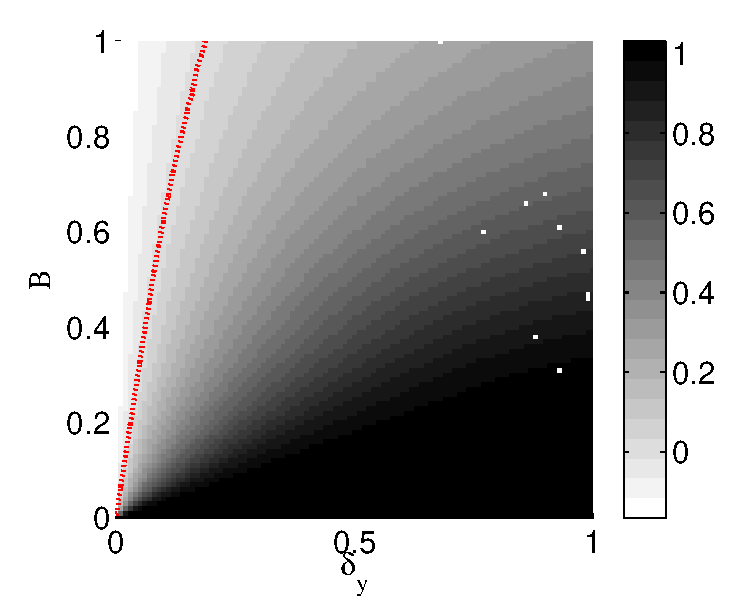
\includegraphics[scale=0.65]{SimpleIRexample_plot.eps}
\caption{(Color available online.) Leaning as a function of both the noise and the y-tolerance.  The red dashed line is the zero contour.  See the text for am explanation of the missing data for large $\delta_y$.}
\end{figure}
\begin{figure}[ht]
\begin{tabular}{cc}
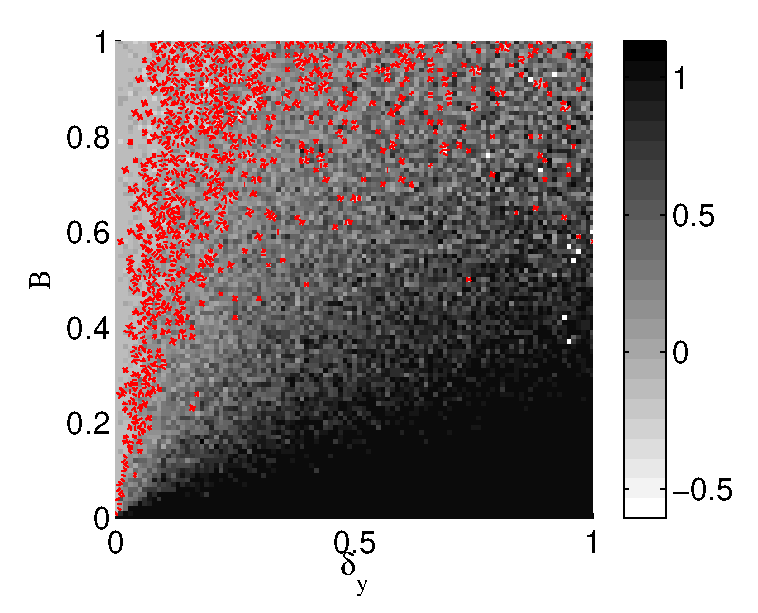
\includegraphics[scale=0.35]{SimpleIRexample_diffLpart1.eps} &
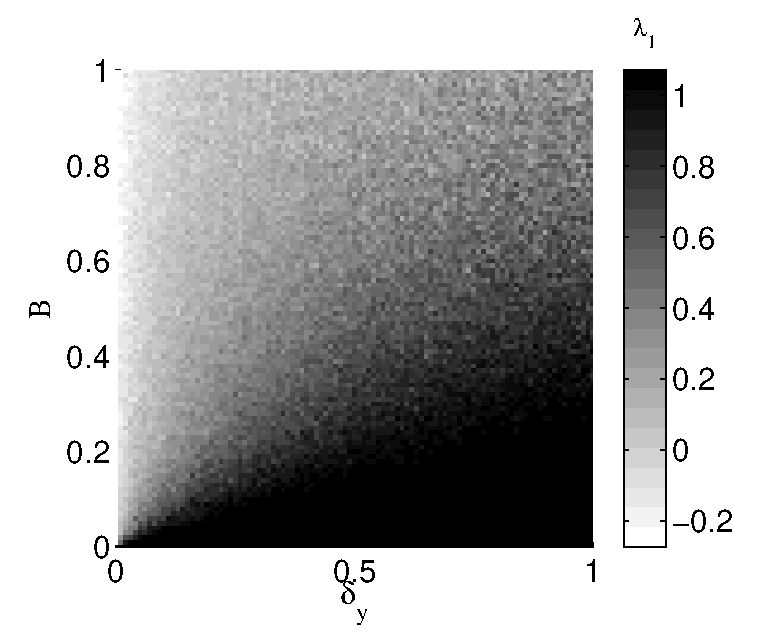
\includegraphics[scale=0.35]{SimpleIRexample_diffLpart2.eps} \\
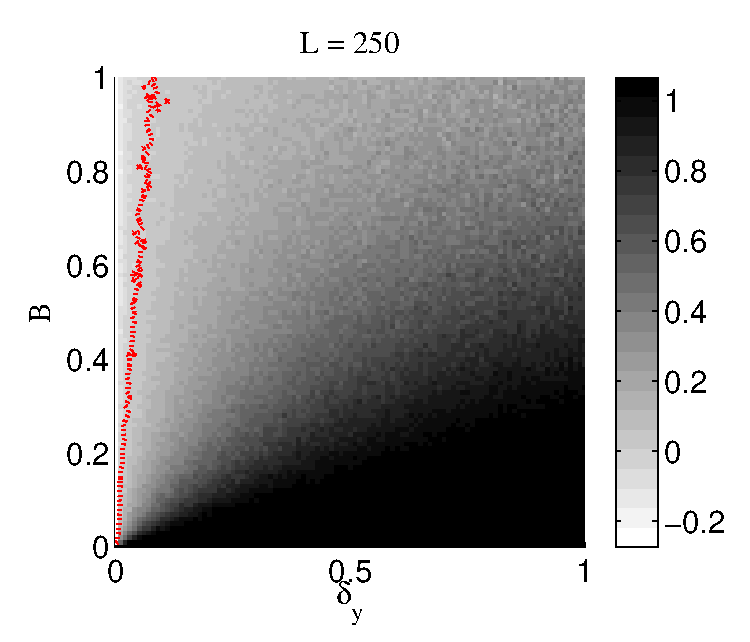
\includegraphics[scale=0.35]{SimpleIRexample_diffLpart3.eps} &
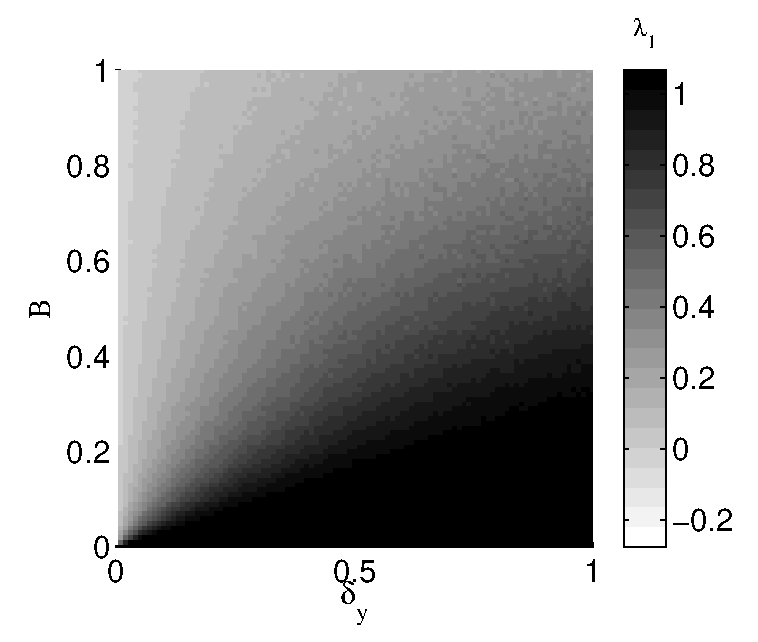
\includegraphics[scale=0.35]{SimpleIRexample_diffLpart4.eps}
\end{tabular}
\caption{(Color available online.) Leaning as a function of both the noise and the y-tolerance for different library lengths.  The red dashed line is the zero contour.  See the text for am explanation of the missing data for large $\delta_y$.}
\end{figure}
\begin{figure}[ht]
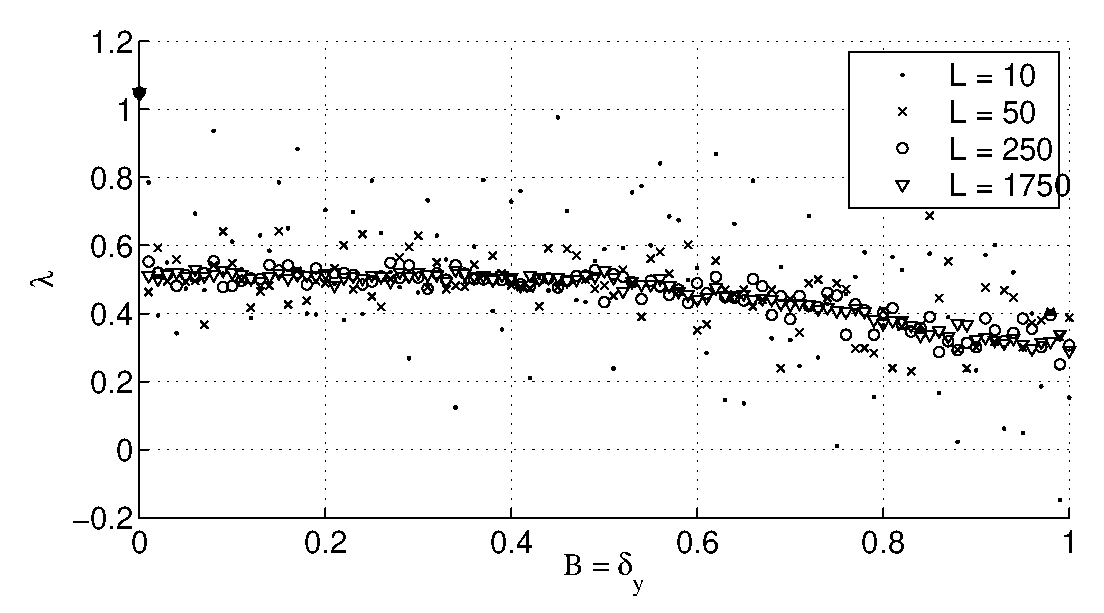
\includegraphics[scale=0.45]{SimpleIRexample_Bxytol.eps}
\caption{(Color available online.) The leaning agrees with intuition for most noise levels when the y-tolerance is set to the noise level (i.e.\ $B=\delta_y$).}
\end{figure}
\begin{figure}[ht]
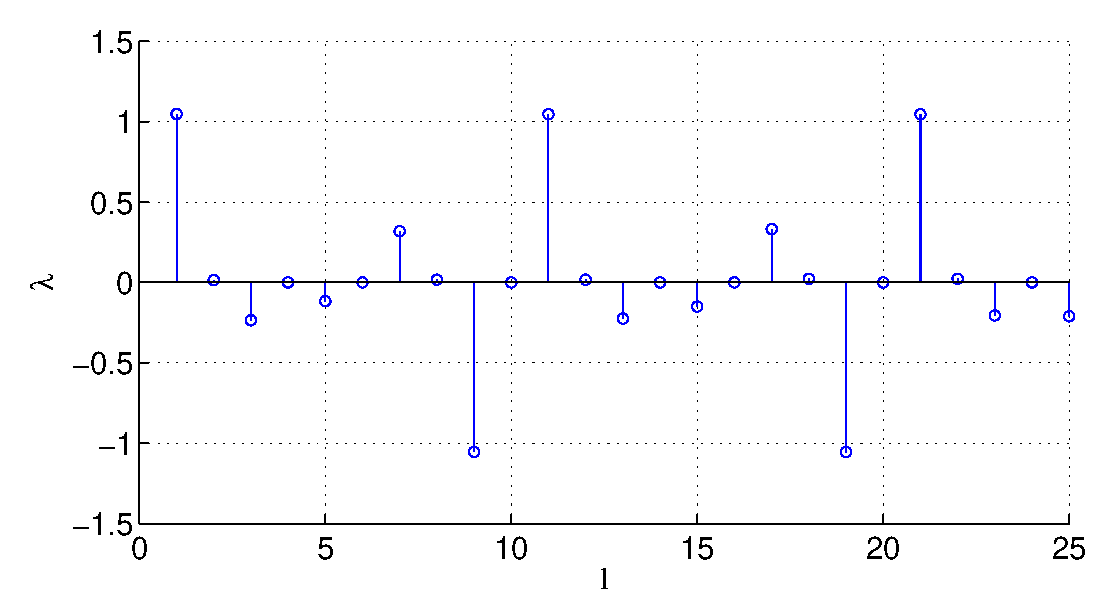
\includegraphics[scale=0.45]{SimpleIRexample_difflags.eps}
\caption{(Color available online.) Different $l$-standard cause-effect assignments lead to different leanings.}
\end{figure}
\begin{figure}[ht]
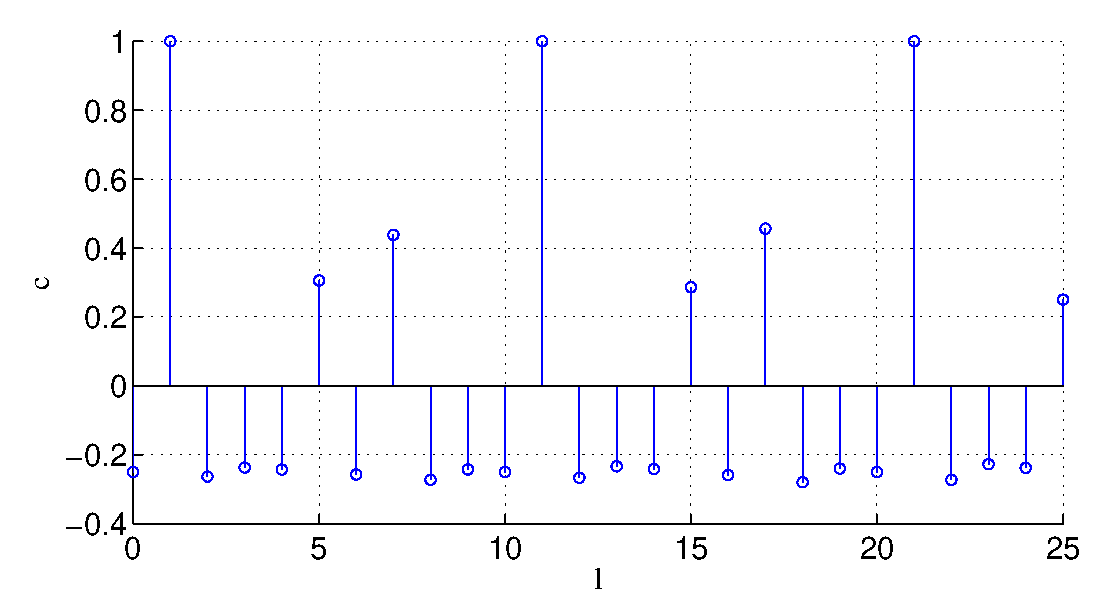
\includegraphics[scale=0.45]{SimpleIRexample_lagcorr.eps}
\caption{(Color available online.) Lagged cross correlations for reference.}
\end{figure}

\subsection{Cyclic Linear Example}
Consider the linear example dynamical system of
\begin{eqnarray}
\label{eq:linearex}
X_t &=& \sin(t)\\
Y_t &=& X_{t-1}+B\eta_t,
\end{eqnarray}
with $B\in\mathbb{R}\ge 0$ and $\eta_t\sim\mathcal{N}\left(0,1\right)$.  Specifically, consider $B\in[0,2]$ in increments of 0.02.  The response system $Y$ is just a lagged version of the driving signal with varying levels of standard Gaussian noise applied at each time step.  

\subsection{Non-Linear Example}
Consider the non-linear dynamical system of
\begin{eqnarray}
\label{eqn:nonlinearEX}
X_t &=& \sin(t)\\
Y_t &=& AX_{t-1}\left(1-BX_{t-1}\right)+C\eta_t,
\end{eqnarray}
with $A,B,C\in\mathbb{R}\ge 0$ and $\eta_t\sim\mathcal{N}\left(0,1\right)$.  Specifically, consider $A,B,C\in[0,5]$ in increments of 0.5.  

\subsection{RL Circuit Example}
\label{sec:rlcirc}
Both of the previous examples included a noise term, $\eta_t$.  Consider a series circuit containing a resistor, inductor, and time varying voltage source related by
\begin{equation}
\label{eqn:it}
\frac{dI}{dt} = \frac{V(t)}{L} - \frac{R}{L} I,
\end{equation}
where $I$ is the current at time $t$, $V(t)= \sin\left(\Omega t\right)$ is the voltage at time $t$, $R$ is the resistance, and $L$ is the inductance.  Eqn. \ref{eqn:it} was solved using the {\em ode45} integration function in MATLAB.  The time series $V(t)$ is created by defining values at fixed points and using linear interpolation to find the time steps required by the ODE solver.  

Consider the situation where $L=10$ Henries and $R=5$ Ohms are constant.  Physical intuition is that $V$ drives $I$, and so we expect to find that $V$ CCM causes $I$ (i.e., $C_{VI}>C_{IV}$ or $\Delta = C_{VI}-C_{IV} > 0$). 


\section{Empirical Data}

\section{Conclusion}

%\bibliographystyle{plain}
%\bibliography{main}

\end{document}